\documentclass[prd,twocolumn,nofootinbib,superscriptaddress,amsmath,amssymb]{revtex4-1}
\usepackage{mathtools}
\usepackage{graphics}
\usepackage{graphicx}
\graphicspath{{./images/}}
\usepackage{dcolumn}
\usepackage{bm}
\usepackage{dsfont} 
\usepackage{amsmath,amssymb}
\usepackage{hyperref}
\usepackage{tabularx}
%\usepackage{epstopdf}
\usepackage{epsf,epsfig}
\usepackage[normalem]{ulem}
\usepackage[usenames]{color}
\usepackage{multirow}
\usepackage{makecell}
\usepackage{diagbox}
\usepackage[abs]{overpic}
%\epstopdfsetup{outdir=./images/}
\allowdisplaybreaks
\hypersetup{
    colorlinks=true,
    linkcolor=blue,
    filecolor=magenta,      
    urlcolor=blue,
    citecolor=blue
}
\urlstyle{same}


\newcommand{\red}[1]{\protect\color{red} #1 \protect\color{black}}
\newcommand{\green}[1]{\protect\color{green} #1 \protect\color{black}}
\newcommand{\blue}[1]{\protect\color{blue} #1 \protect\color{black}}
\newcommand{\black}[1]{\protect\color{black} #1 \protect\color{black}}
\newcommand{\yellow}[1]{\protect\color{yellow} #1 \protect\color{black}}
\newcommand{\bra}[1]{\protect\langle #1 |}
\newcommand{\ket}[1]{| #1 \protect\rangle}
\newcommand{\braket}[2]{\protect\langle #1 | #2 \protect\rangle}
\newcommand{\expected}[1]{\protect\langle #1 \protect\rangle}
\newcommand{\R}{{\mbox{\tiny R}}}
\newcommand{\ky}[1]{\textcolor{blue}{\it{\textbf{ky: #1}}} }
\newcommand{\kent}[1]{\textcolor{magenta}{\textbf{ #1}} }
\newcommand{\zack}[1]{\textcolor{magenta}{\textbf{ #1}} }
\newcommand{\zc}[1]{\textcolor{red}{\it{\textbf{zc: #1}}} }
\definecolor{red(ncs)}{rgb}{0.77, 0.01, 0.2}
\newcommand{\ny}[1]{\textcolor{blue}{NY: #1} }
\newcommand{\kc}[1]{\textcolor{green}{KC: #1} }
\newcommand{\NS}{{\mbox{\tiny NS}}}
\newcommand{\sci}[2]{#1 \times 10^{#2}}

\usepackage{array}
\newcolumntype{C}[1]{>{\centering\let\newline\\\arraybackslash\hspace{0pt}}m{#1}}


\newcolumntype{C}[1]{>{\centering\arraybackslash}m{#1}}

\def\eq#1{Eq.~(\ref{eq:#1})}
\def\Eq#1{Equation~(\ref{eq:#1})}
\def\eqs#1#2{Eqs.~(\ref{eq:#1}) \& (\ref{eq:#2})}
\def\eqlist#1#2{Eqs.~(\ref{eq:#1}-\ref{eq:#2})}
\def\Eqs#1#2{Equations~(\ref{eq:#1}) \& (\ref{eq:#2})}
\def\Eqlist#1#2{Equations~(\ref{eq:#1}-\ref{eq:#2})}
\def\fig#1{Fig.\ref{fig:#1}}
\def\figs#1#2{Figs.\ref{fig:#1} \& \ref{fig:#2}}
\def\Fig#1{Figure~\ref{fig:#1}}
\def\Figs#1#2{Figures~\ref{fig:#1} \& \ref{fig:#2}}
\def\tab#1{Table~\ref{tab:#1}}
\def\sec#1{Section~\ref{sec:#1}}



\begin{document}

\title{Universal relations after GW170817}

\author{Zachary Carson}
\affiliation{%
 Department of Physics, University of Virginia, Charlottesville, Virginia 22904, USA
}%

\author{Katerina Chatziioannou}
\affiliation{%
 Canadian Institute for Theoretical Astrophysics, 60 St. George Street, Toronto, Ontario, M5S 3H8, Canada
}%
\affiliation{%
 Center for Computational Astrophysics, Flatiron Institute, 162 5th Ave, New York, NY 10010
}%

\author{Carl-Johan Haster}
\affiliation{%
 Canadian Institute for Theoretical Astrophysics, 60 St. George Street, Toronto, Ontario, M5S 3H8, Canada
}%
\affiliation{%
 Center for Computational Astrophysics, Flatiron Institute, 162 5th Ave, New York, NY 10010
}%

\author{Nicol\`as Yunes}
\affiliation{%
 Department of Physics, Montana State University, Bozeman, MT 59717, USA.
}%
\affiliation{%
 Department of Physics and MIT Kavli Institute,
}%

\author{Kent Yagi}
\affiliation{%
 Department of Physics, University of Virginia, Charlottesville, Virginia 22904, USA
}%


\date{\today}

%%%%%%%%%%%%%%%%%%%%%%%%%%%%%%%% Begin Abstract %%%%%%%%%%%%%%%%%%%%%%%%%%%%%%%%%%%%%%%%%%%%%%%%%%%%%%%%%%%%%%%%%%%%%%%%%%%%%%%%%%%%%%%%%%%%%%%%%%%%%%%%%%%%%%%%%%%%%%%%%%%%%%%%%%%%%%%%%%%%%%%%%%%%%%%%%%%%%
\begin{abstract}
% Intro
The thermodynamic relationship between pressure and density (the equation of state) of supranuclear matter, accessible primarily in neutron stars, is critical to the study of such stars, and is one of the largest uncertainties in nuclear physics to date. 
% How to probe
The extraction of tidal deformabilities from the gravitational waveforms of binary neutron star merger events, such as GW170817, is a promising method of probing the nuclear structure.
% What was done before - Binary Love
Previous studies have shown that approximately equation of state insensitive ``binary Love universal relations" exist between symmetric and antisymmetric combinations of individual tidal deformabilities, which are difficult to be independently measured with second-generation gravitational wave interferometers.
% What was done before - I-Love-Q
Similarly, another set of equation of state independent relations exist between individual neutron star parameters: moment of inertia (I), tidal deformability (Love number), and quadrupole moment (Q) - known as the ``I-Love-Q universal relations."
% What universal relations do
Such universal relations allow the elimination of some tidal parameters from the list of model parameters, thus breaking degeneracies and ultimately reducing the uncertainty of the dominant tidal effect in parameter estimation.
% What we will do
In this document, we explain how one can reduce equation of state variation for both binary Love and I-Love-Q universal relations, which helps to reduce systematic errors on the tidal measurement of binary neutron star mergers. 
We achieve this  by restricting to only equations of state drawn from the 90\% posterior constraint on pressure as a function of density, as derived by the LIGO Collaboration.
% What we found
We find an improvement in binary Love universality by a factor of $\sim 59$\% for stars with a mass ratio of 0.75, and in I-Love-Q universality by factors of $\sim 50$\%.
% Conclude
We end by comparing systematic errors on tidal measurement due to the equation of state variation with statistical errors and comment on whether one can safely use these universal relations with future gravitational wave observations.
\end{abstract}

\maketitle

%%%%%%%%%%%%%%%%%%%%%%%%%%%%%%% Begin Introduction %%%%%%%%%%%%%%%%%%%%%%%%%%%%%%%%%%%%%%%%%%%%%%%%%%%%%%%%%%%%%%%%%%%%%%%%%%%%%%%%%%%%%%%%%%%%%%%%%%%%%%%%%%%%%%%%%%%%%%%%%%%%%%%%%%%%%%%%%%%%%%%%%%%%%%%%%%%%%%

\section{Introduction}\label{sec:intro}
%Intro
The dependence of pressure on density for supranuclear matter found primarily inside neutron stars (NSs) remains to be one of the largest mysteries in both nuclear physics and astrophysics.
This internal structure of such stars, known as the equation of state (EoS), is exceedingly important, as it is the determining factor for many NS observables - such as the mass, the radius, and many more.
Unfortunately, terrestrial experiments can only study the EoS up to the nuclear saturation density ($\rho_{\text{sat}} \approx 2.5 \times 10^{14} \text{ g/cm}^3$)~\cite{Li:HeavyIon,Tsang:SymmetryEnergy,Centelles:NeutronSkin,Li:CrossSections,Chen:SymEnergy}, making NSs ideal laboratories for constraining ultra dense nuclear matter.

%Constraining the EoS
Independent measurements of NS observables can be used to constrain the nuclear EoS.
For example, electromagnetic observations of the mass-radius relationship of NSs have been used to place limits on NSs~\cite{guver,ozel-baym-guver,steiner-lattimer-brown,Lattimer2014,Ozel:2016oaf}.
However, these implications suffer from large systematic errors due to astrophysical mismodeling.
Alternatively, the emission of gravitational waves (GWs) from binary NS merger events have proven to be a unique method of probing nuclear physics.
During the early inspiral portion of the merger, the orbital separation is large enough that the effect of companion tidal fields is negligible. 
As the separation decreases through GW emission, tidal forces are magnified and the NSs deform from sphericity, altering the orbital trajectories; a relic which is directly imprinted on the GW signal.
This deformation is characterized by the \textit{tidal deformability} $\Lambda$ as the linear response of the NSs quadrupole moment $Q_{ij}$ to the neighboring tidal field $\varepsilon_{ij}$.

%reparameterization of the template
In the case of binary NSs, each star becomes deformed via the process highlighted above, resulting in two highly correlated tidal parameters $\Lambda_1$ and $\Lambda_2$ entering in the gravitational waveform.
Due to high correlations between between the two parameters, independent extraction becomes very difficult at current interferometer sensitivities.\zc{cite?}
Typically, these high correlations can be reduced by strategically reparameterizing the waveform template with new tidal parameters constructed from linear combinations of $\Lambda_1$ and $\Lambda_2$.
For example, utilizing the parameters $\tilde{\Lambda}$ and $\delta \tilde{\Lambda}$~\cite{hinderer-love,Flanagan2008} which enter the GW waveform at different post-Newtonian (PN) orders (powers of the ratio between the orbital speed and the speed of light $v/c^{2n}$) partially mitigates these correlations.

%Universal relations
Unfortunately, current detectors are only sensitive enough to accurately measure the dominant tidal parameter, $\tilde{\Lambda}$, known as the chirp deformability.
Previous work by Yagi and Yunes~\cite{Yagi:binLove} resolved this issue by finding approximately EoS-insensitive ``binary Love universal relations" between symmetric and anti-symmetric combinations of tidal deformabilities $\frac{1}{2}(\Lambda_1 \pm \Lambda_2)$.
This allows one to further break degeneracies between tidal parameters, resulting in both (i) a decrease in uncertainty upon parameter extraction on the removal of one parameter from the model, and (ii) the ability to measure the secondary tidal parameter upon measurement of the first.  
This important work showed up to an order of magnitude improvement in parameter estimation through a simple Fisher analysis.
Similar ``I-Love-Q" universal relations~\cite{Yagi:ILQ} have been found between individual NS observables: quadrupole moment , moment of inertia, and tidal deformability; similarly allowing the removal of tidal parameters from the model list, and allowing an automatic determination of one observable through the measurement of another.

%How we improved this
In this analysis, we aim to improve this important work by imposing the restrictions found on the EoS~\cite{LIGO:posterior} derived from the recent binary NS merger observation, GW170817~\cite{TheLIGOScientific:2017qsa}.
By restricting to only EoSs which lie within the the 90\% credible region on pressure as a function of density found in~\cite{LIGO:posterior}, we repeat the analyses done in~\cite{Yagi:binLove,Yagi:ILQ} and show an increase in universality for both binary Love and I-Love-Q universal relations.
In addition, we consider hybrid star EoSs seen in~\cite{Paschalidis2018}, which experience strong first-order transitions from hadronic matter to quark matter.
These provide a departure from the nuclear matter relations considered here - providing valuable insight into them.
Further, we estimate the viability of using improved universal relations on future GW detections by performing simple Fisher analyses to approximate when the statistical errors from parameter extraction become comparable to the systematic errors due to EoS variation in universal relations.

\subsection{Executive Summary}
%What we did
In this paper we attempt to improve binary Love and I-Love-Q universal relations by imposing constraints on the EoS found by GW170817~\cite{LIGO:posterior,TheLIGOScientific:2017qsa}.
First, we generate two large samples of spectral EoSs~\cite{Lindblom:2018rfr}, where we (i) impose the restriction that they must be drawn from GW170817s 90\% credible posterior in pressure as a function of density, and (ii) don't impose any restrictions for comparison purposes.
Next, we follow the important works of~\cite{Yagi:binLove} and~\cite{Yagi:ILQ} to show how the ``constrained" set of EoSs show improved universality from both the previous works, and the ``unconstrained" sample, shown by Fig.~\ref{fig:ILQ}.
In addition, we determine the degree to which hybrid star EoSs obey binary Love universal relations.
Finally, through a simple Fisher analysis, we consider the value in improving universal relations by approximating when the statistical errors from parameter extraction become comparable to the systematic errors due to EoS variation in universal relations.

%Final Results
Upon use of the constrained set of EoSs, we find an improvement in binary Love universality by a factor of $\sim 59$\% for stars with mass ratios of $0.75$, and in I-Love-Q universality by factors of $\sim50$\%, tabulated in Tab.~\ref{tab:maxVar}.
We also find that binaries consisting of one massive hybrid star, and one small-mass hadronic star do not agree with derived binary Love relations, due to the large separation in $\tilde{\Lambda}$ between the constituent stars.
Unfortunately, due to the current limitations in detector sensitivity, the systematic errors arising from EoS variation in the universal relations are far outweighed by the statistical errors accrued by extraction of high-order PN tidal parameters from GW waveforms.
Fig.~\ref{fig:stackedFisher} compiles the results from Fisher analyses approximating the uncertainties accrued from parameter extraction for GW170817 as if it had been observed by future detectors $A \equiv ($ O2, aLIGO, a\texttt{++}, Voyager, ET, CE$)$\zc{cite these individually}.
Here, $\sigma^A_{\text{GW170817}}$ and $\rho^A_{\text{GW170817}}$ correspond to the statistical error and signal-to-noise-ratio found from observing GW170817 on detector $A$, and $\sigma^A_N$ represents the combined uncertainty after the detection of $N_A$ events (corresponding to the binary NS merger rate associated interferometer $A$).
These values are further tabulated in Table~\ref{tab:variances}.
It can be seen from this figure that the statistical errors from parameter extraction become comparable the universal relation systematics (indicated by the magenta horizontal line) for the Voyager telescope - indicating when improved binary Love universal relations will become viable.
\begin{figure}
\begin{center} 
\includegraphics[width=\columnwidth]{stackedFisher.eps}
\end{center}
\caption{
Estimated statistical uncertainties $\sigma^A_{\text{GW170817}}$ (blue) in the extraction of $\tilde{\Lambda}$ from GW170817 (O2) as if observed with future interferometers aLIGO, a++, Voyager, CE, and ET-D as a function of the signal-to-noise-ratio $\rho^A_{\text{GW170817}}$.
This is compared to the combined uncertainty $\sigma^A_N$ (red) from the observation of multiple events from a simulated population of size $N_A$ corresponding to the upper (teal), central (orange), and lower (magenta) limits of expected binary NS merger detection rates for O2, aLIGO, a\texttt{++}, Voyager, CE, and ET-D over 1 observation year.
It can be seen that the statistical errors in parameter extraction become comparable to the systematics from EoS variation in binary Love relations (purple) for Voyager and on.
Note there is no simulated populations of events under the O2 design sensitivity - due to there only being a single event during the observing period.
These results are further tabulated in Table~\ref{tab:variances}.
}
\label{fig:stackedFisher}
\end{figure} 

%outline
The organization of this paper is outlined below.
We begin with a complementary background and theory material in Sec.~\ref{sec:theory}.
We continue in Sec.~\ref{sec:universal} by finding new and improved binary Love and I-Love-Q universal relations, and considering how well hybrid star EoSs agree with the universal relations.
We next examine these improved universal relations and question whether or not they are useful for future interferometers in Sec.~\ref{sec:observations}.
We conclude in Sec.~\ref{sec:conclusion} by discussing our results and mentioning avenues of future work.
Throughout this paper, we have adopted geometric units of $G=c=1$, unless otherwise stated.

%%%%%%%%%%%%%%%%%%%%%%%%%%%%%%%%% Begin theory %%%%%%%%%%%%%%%%%%%%%%%%%%%%%%%%%%%%%%%%%%%%%%%%%%%%%%%%%%%%%%%%%%%%%%%%%%%%%%%%%%%%%%%%%%%%%%%%%%%%%%%%%%%%%%%%%%%%%%%%%%%%%%%%%%%%%%%%%%%%%%%%%%%%%%%%%%%%
\section{Background and theory}\label{sec:theory}

\subsection{Spectral representations of neutron star equations of state}\label{sec:eos}
The structure of a NS and its tidal interactions in a binary system rely heavily on the underlying state function describing the relationship between pressure ($p$) and energy density ($\epsilon$), or equation of state, of nuclear matter.
Given that all currently proposed EoSs utilize certain approximations, one method to study a wide range of physically realizable EoSs is to parameterize them in a model-independent way.
Spectral representations~\cite{Lindblom:2010bb,Lindblom:2012zi,Lindblom:2013kra,Lindblom:2018rfr,Abbott:2018exr} parameterize EoSs by performing spectral expansions on the adiabatic index $\Gamma(p)$\footnote{Another way of parameterizing EoSs is the piecewise polytropic formulation~\cite{Read2009,Lackey:2014fwa,Carney:2018sdv}.}:
\begin{equation}
\Gamma(x) = \exp{\sum_k\gamma_k x^k},
\end{equation}
where $x \equiv \log{p/p_0}$ for minimum pressure $p_0$.
The equation of state is then determined by an integration of the differential equation:
\begin{equation}
\frac{d \epsilon(p)}{dp}=\frac{\epsilon(p)+p}{p \Gamma(p)}.
\end{equation}
Using this formalism, any valid EoS can be approximated through choice of 4 or more spectral coefficients $\gamma_k$, tabulated for several common EoSs in Table 1 of~\cite{Lindblom:2018rfr}.

In the current analysis, we consider EoSs which have been constrained by the recent binary neutron star merger event, GW170817.
Important recent work~\cite{LIGO:posterior} sampled EoS parameters in order to derive a marginalized posterior on the pressure as a function of mass density, as seen in Fig. 2 of~\cite{LIGO:posterior}.
The spectral coefficients were sampled within the ranges: $\gamma_0 \in \lbrack 0.2,2 \rbrack$, $\gamma_1 \in \lbrack -1.6,1.7 \rbrack$, $\gamma_2 \in \lbrack -0.6,0.6 \rbrack$, $\gamma_0 \in \lbrack -0.02,0.02 \rbrack$, and further restricted the adiabatic index to be $\Gamma \in \lbrack 0.6,4.5 \rbrack$, ensuring the parameterization exposed a wide range of viable EoSs~\cite{Lindblom:parameters}.
Additional constraints imposed upon the generated EoSs were as follows~\cite{LIGO:posterior}: (i) causality within 10\%, and (ii) EoS priors must support NS masses up to $1.97 \text{ M}_{\odot}$, consistent with astrophysical observations.
We utilize a random set of 100 of the above posterior samples defined by GW170817, furthermore referenced as the ``constrained EoSs", as shown in Fig.~\ref{fig:eos}.\zc{Carl, can you describe how you generated these? They aren't the \emph{actual} posteriors, are they?}
Following~\cite{Read2009}, the parameterized high-density core EoSs generated above are matched to the low-density crust EoS Sly~\cite{Douchin:2001sv} at about half of the nuclear saturation density, $\rho_{\text{stitch}}=1.3 \times 10^{14} \text{ g/cm}^3$.
For comparison, we also include a second sample of 100 ``unconstrained" EoSs, randomly sampled in the pressure-density plane to be unrestricted by GW170817s posterior.

In addition, we investigate 10 transitional quark-hadron matter stars, which undergo first-order phase transitions at pressure $P_{\text{tr}}$, where the hadronic branch departs into a quark-matter branch at a given mass transition~\cite{Paschalidis2018,Alford:2017qgh,1971SvA....15..347S,Zdunik:2012dj,Alford:2013aca}.
In particular, we focus on the ACS and ACB models described in Ref.~\cite{Paschalidis2018}, shown in Fig.~\ref{fig:hybridML}.
These result in two distinct types of NSs, based on their observed mass: (i) massive ($M \geq \text{ M}_{\text{tr}}$) hybrid stars which have quark-matter cores and nuclear matter crusts (we denote this as ``HS"), and (ii) small-mass ($M \leq \text{ M}_{\text{tr}}$) hadronic stars with no internal transition to quark matter (we denote this as ``NS").

\begin{figure}
\begin{center} 
\includegraphics[width=\columnwidth]{EoSs.eps}
\end{center}
\caption{
Small representative sets of the constrained (left) and unconstrained (right) EoSs used in this analysis. 
The constrained EoSs were populated by randomly selecting 100 posterior samples obtained from the GW170817 90\% credible level shown in cyan~\cite{LIGO:posterior}.
Additionally, 100 unconstrained EoSs were generated by randomly sampling spectral coefficients of physically valid EoSs, with no further constrained applied.
The following constraints were also applied to both sets of EoSs: (i) the EoS must have a causal structure within 10\%, and (ii) the EoS must support maximum NS mass of at least $1.97 \text{ M}_{\odot}$, consistent with astrophysical observations.
Finally, the high density core EoSs generated above were stitched to the low-density crust EoS of SLy~\cite{Douchin:2001sv} at $\rho_{\text{stitch}}=1.3 \times 10^{14} \text{ g/cm}^3$.
}
\label{fig:eos}
\end{figure} 

\begin{figure}
\begin{center} 
\includegraphics[width=\linewidth]{hybridML.eps}
\end{center}
\caption{
$M-\Lambda$ relations for the ACS and ACB class model hybrid stars. 
Observe the transitional points where the NS transitions from the hadronic branch into a quark-matter branch.
As described in the text, HS/HS and NS/NS binaries have individual masses chosen such that both stars are contained within one branch -- resulting in high $q$ values.
Constrastingly, HS/NS binaries have individual masses chosen from each branch resulting in small $q$-values.
}
\label{fig:hybridML}
\end{figure} 

\subsection{Neutron Star Tidal deformability}\label{tidal}
Binary neutron star mergers, such as GW170817, provide valuable insight into the internal structure of such stars. 
Namely, tidal effects which enter the gravitational waveform depend strongly on the EoS defining the NSs structure. 
The ($l=2$ electric type) \emph{tidal deformability}, denoted as $\lambda$, has the largest impact on the waveform phase. 
Consider a NS of mass $M$ in the presence of the tidal field $\varepsilon_{ij}$ of a companion star.
In response, the NS will deform away from sphericity under the acquisition of quadrupole moment $Q_{ij}$, characterized by $\lambda$ as the linear response to $\varepsilon_{ij}$~\cite{Flanagan2008,hinderer-love,Yagi2013}:
\begin{equation}
Q_{ij}=-\lambda \varepsilon_{ij}.
\end{equation}
One can extract $Q_{ij}$ and $\varepsilon_{ij}$ -- and thus $\lambda$, or its dimensionless form $\Lambda \equiv \lambda/M^5$ -- via diffent asymptotic limits of the gravitational potential:
\begin{align}
\begin{split}
\Phi=\frac{1+g_{tt}}{2}&=-\frac{M}{r} - \frac{3}{2}\frac{Q_{ij}}{r^3} \Bigg(\frac{x^i}{r} \frac{x^j}{r}-\frac{1}{3}\delta_{ij} \Bigg) + \mathcal{O} \Bigg( \frac{M^4}{r^4} \Bigg)\\
&+ \frac{1}{2} \varepsilon_{ij} x^i x^j + \mathcal{O} \Bigg( \frac{r^3}{M^3} \Bigg).
\end{split}
\end{align}
The metric component $g_{tt}$ is determined by first constructing a spherically symmetric, non-spinning background solution, followed by the introduction of a perturbative tidal deformation.
Next, the perturbed Einstein equations must be solved in the NSs interior given an EoS, then matched to the exterior Schwarzschild solution at the surface, modulo a constant.
This process is described in more detail in Ref.~\cite{hinderer-love}.
Further, the stellar mass and radius are determined from $p(R)=0$, and the above mentioned constant.
Similarly, the moment of inertia is obtained from the asymptotic behavior of the $g_{t \phi}$ metric component.

Next, we consider the case of two NSs in a binary, such as the system found in GW170817, where each star 
individually experiences a neighboring tidal field.
Thus each star possesses tidal deformabilities $\Lambda_1$ and $\Lambda_2$ entering the gravitational waveform.
Due to strong correlations between these parameters, individual extraction is very difficult with current interferometer sensitivity limitations.
However, the waveform templates can be strategically reparameterized to instead include independent linear combinations of $\Lambda_1$ and $\Lambda_2$ to mitigate correlations between them. 
Any set of two independent functions may be used, for example: tidal parameters $\tilde{\Lambda}=\tilde{\Lambda}(\Lambda_1,\Lambda_2)$ and $\delta \tilde{\Lambda}=\delta \tilde{\Lambda}(\Lambda_1,\Lambda_2)$~\cite{Wade:tidalCorrections} first enter the gravitational waveform at 5PN and 6PN orders respectively, thus partially breaking degeneracies.
Here, $\tilde{\Lambda}$ is known as the mass weighted tidal deformability, or \emph{chirp deformability} due to its status as the dominant tidal parameter in the waveform. 

\subsection{EoS insensitive relations}\label{sec:eosInsensitive}
Current gravitational wave interferometry is not yet sensitive enough to accurately extract both tidal parameters $\tilde{\Lambda}$ and $\delta\tilde{\Lambda}$.
In a search to remedy this, important previous work by Yagi and Yunes~\cite{Yagi:binLove} found that symmetric and antisymmetric combinations of tidal deformabilities:
\begin{equation}
\Lambda_s \equiv \frac{\Lambda_1 + \Lambda_2}{2}, \hspace{6mm} \Lambda_a \equiv \frac{\Lambda_1 - \Lambda_2}{2},
\end{equation}
display EoS-insensitive properties to a high degree, showing EoS variations up to 20\% for binaries with masses less than $1.7 \text{ M}_{\odot}$, for a representative set of 11 EoSs. 
These relations, known as ``binary Love universal relations" allows one to break degeneracies between coupled tidal parameters.
This is important for two reasons: (i) allows us to algebraically eliminate tidal parameters from the template parameter list, improving parameter estimation, and (ii) automatic measurement of second tidal parameter given observation of the first.
It was shown through a simple Fisher analysis that the use of binary Love universal relations improved parameter extraction on $\tilde{\Lambda}$ by an order of magnitude.

Similar universal relations have been found to exist between individual NS observables: moment of inertia (I), tidal deformability (Love), and quadrupole moment (Q), known as the ``I-Love-Q" universal relations~\cite{Yagi:ILQ}.
These have been found to be EoS insensitive by up to 1\% for each of pair of observables.
In this paper, we show improvement in both of these universal relations by restricting to EoSs sampled from GW170817s posterior on pressure as a function of density.
%%%%%%%%%%%%%%%%%%%%%%%%% Begin universal relations %%%%%%%%%%%%%%%%%%%%%%%%%%%%%%%%%%%%%%%%%%%%%%%%%%%%%%%%%%%%%%%%%%%%%%%%%%%%%%%%%%%%%%%%%%%%%%%%%%%%%%%%%%%%%%%%%%%%%%%%%%%%%%%%%%%%%%%%%%%%%%%%%%%%%
\section{Universal relations}\label{sec:universal}
In this section, we follow the analyses performed in~\cite{Yagi:binLove,Yagi:ILQ} with two new sets of 100 spectrally generated EoS: (i) posterior samples randomly selected from GW170817s 90\% posterior on on pressure as a function of density as shown in the left panel of Fig.~\ref{fig:eos}, and (ii) those unconstrained by any prior EoS information, as shown in the right panel of Fig.~\ref{fig:eos}.

\subsection{I-Love-Q relations}\label{sec:ilq}
Here we present our results on I-Love-Q universality as compared to Fig. 1 of Yagi and Yunes~\cite{Yagi:ILQ}.
In particular, we consider two distinct classes of NSs: nuclear matter EoSs and hybrid quark-hadron star EoSs as described in Sec.~\ref{sec:theory}.
We begin in Sec.~\ref{sec:ilq-nuc} by fitting the new I-Love-Q universal relations using the constrained set of EoSs.
This is followed in Sec.~\ref{sec:ilq-hyb} by an analysis and discussion into how well hybrid stars agree with the improved binary Love relations. 

\subsubsection{Nuclear matter stars}\label{sec:ilq-nuc}
Following the work of Ref.~\cite{Yagi:ILQ}, the data for each universal relation is first fit to the following curve:
\begin{equation}\label{eq:ILQfit}
\ln{y_i}=a_i+b_i \ln{x_i} + c_i (\ln{x_i})^2 + d_i (\ln{x_i})^3 + e_i (\ln{x_i})^4,
\end{equation}
where the updated coefficients are given in Table~\ref{tab:ILQfit}.
Additionally, we offer an improvement to the functional form of the I-Love-Q fitting curve. 
Namely, we use the Newtonian relationships between various observables as a controlling factor in the fit~\cite{Yagi:ILQ}:
\begin{equation}\label{eq:Newtonian}
\bar{I}^{\text{N}} = C_{\bar{I}\Lambda}\Lambda^{2/5}, \hspace{3mm} \bar{Q}^{\text{N}} = C_{\bar{Q}\Lambda}\Lambda^{1/5}, \hspace{3mm} \bar{I}^{\text{N}} = C_{\bar{I}\bar{Q}}\bar{Q}^{2}.
\end{equation}
This is appended to an expansion in $\Lambda^{-1/5} \propto C$ (or $\bar{Q}^{-1/5}$), where $C=M/R$ is the compactness of the star.
This results in the following overall fitting relation:
\begin{equation}\label{eq:ILQfitNew}
y=C_{yx} x^{\alpha} \frac{1+\sum_{i=1}^3 a_i x^{-i/5}}{1+\sum_{i=1}^3 b_i x^{-i/5}},
\end{equation}
where $y$ and $x$ correspond to NS observables $\bar{I}$, $\bar{Q}$, and $\Lambda$, and $\alpha$ is given by $2/5$, $1/5$, and $2$ for the $\bar{I}-\Lambda$, $\bar{Q}-\Lambda$, and $\bar{I}-\bar{Q}$ relations, respectively.
The new fitting coefficients are presented in Table~\ref{tab:ILQfitNew}.
While the two above fits both result in fits with similar $R^2$ values of $\sim 0.9999995$ for the data presented, the lattter one has the advantage that it properly limits to the Newtonian case as $\Lambda \rightarrow \infty$~\cite{Yagi:binLove}.

\begin{table*}
\centering
\caption{
Updated fit parameters for the I-Love-Q universal relations, fitted to the constrained EoS data by the curve found in Eq.~\ref{eq:ILQfit}.
}\label{tab:ILQfit}
\begin{tabular}{ c  c | c c c c c } 
 \hline
 \hline
 $y_i$ & $x_i$ & $a_i$ & $b_i$ & $c_i$ & $d_i$ & $e_i$ \\
 \hline
 $\bar{I}$ & $\Lambda$ & $1.4934168$ & $0.0640972$ & $0.0208513$ & $-5.018022 \times 10^{-4}$ & $3.1638958 \times 10^{-7}$ \\
 $\bar{Q}$ & $\Lambda$ & $0.2092931$ & $0.0740442$ & $-0.0538210$ & $-5.018022 \times 10^{-3}$ & $1.576165 \times 10^{-4}$ \\ 
  $\bar{I}$ & $\bar{Q}$ & $1.3832702$ & $0.0.5931020$ & $-0.0216132$ & $0.0419044$ & $-2.9676365 \times 10^{-3}$ \\
 \hline
 \hline
\end{tabular}
\end{table*}

\begin{table*}
\centering
\caption{
I-Love-Q universal relations fit parameters for the constrained EoS data using the improved fitting relations found in Eq.~\ref{eq:ILQfitNew}.
This fitting relation, unlike previous versions, properly limits to the Newtonian case as $\Lambda \rightarrow \infty$.
}\label{tab:ILQfitNew}
\begin{tabular}{ c  c  | c c c c c c c c} 
 \hline
 \hline
 $y$ & $x$ & $\alpha$ & $C_{yx}$ & $a_1$ & $a_2$ & $a_3$ & $b_1$ & $b_2$ & $b_3$ \\
 \hline
 $\bar{I}$ & $\Lambda$ & $2/5$ & $0.5313031$ & $1.2868285$ & $0.0988787$ & $-2.3001034$ & $-1.3465945$ & $0.3857349$ & $-0.0287014$\\
 $\bar{Q}$ & $\Lambda$ & $1/5$ & $3.5554627$ & $-2.1218079$ & $2.7237378$ & $-1.4906808$ & $0.8643535$ & $-0.1427541$ & $-1.3973147$\\
 $\bar{I}$ & $\bar{Q}$ & $2$ & $0.0089212$ & $10.5910815$ & $-37.4581345$ & $43.1831156$ & $-2.3610288$ & $1.9674667$ & $-0.5678018$\\
\hline
\hline
\end{tabular}
\end{table*}

Fig.~\ref{fig:ILQ} shows the improved I-Love universal relations between the dimensionless moment of inertia $\bar{I} \equiv I/M^3$, the dimensionless quadrupole moment $\bar{Q} \equiv Q/M^3$, and the dimensionless tidal deformability $\Lambda$ for both the constrained and unconstrained sets of EoSs (each with individual fits pertaining to only that set of EoSs).
We observe that the constrained EoSs show considerable improvement from both the results of previous works~\cite{Yagi:ILQ}, and from the unconstrained EoSs.
This is further validated in Tab.~\ref{tab:maxVar}, where the maximal EoS variation from each fit is tabulated; comparing the results of previous works to the unconstrained, and constrained sets of EoSs.
Observe how the constrained EoSs outperform both other cases by a considerable amount for each I-Love-Q universal relation.

\begin{figure*}
\begin{center} 
\includegraphics[width=.32\textwidth]{IL.eps}
\includegraphics[width=.32\textwidth]{QL.eps}
\includegraphics[width=.32\textwidth]{IQ.eps}
\end{center}
\caption{
Individual I-Love universal relations $\bar{I}-\Lambda$ (left), $\bar{Q}-\Lambda$ (center), and $\bar{I}-\bar{Q}$ (right), shown for both the constrained EoSs (solid green) and unconstrained EoSs (dotted maroon).
In these figures, the black dashed lines corresponds to the fits given by Eq.~\ref{eq:ILQfitNew} (note: each panel contains individual fits for the constrained and unconstrained EoSs, indistinguishable on such a large scale).
Observe how the fractional difference from the fits, shown in the bottom panels, is greatly suppressed for the constrained case, compared to both the unconstrained case, and results from previous works~\cite{Yagi:ILQ}.
The maximal EoS variation from the fits for the unconstrained and constrained sets of EoSs are compared in Tab.~\ref{tab:maxVar}.
Additionally shown in this figure is the fractional difference from the nuclear matter fits for the 10 hybrid star EoSs (dashed green).
}
\label{fig:ILQ}
\end{figure*} 


\begin{table}
\centering
\caption{
Comparison between the universal relations (both I-Love-Q and binary Love) maximal EoS variability for the results of previous works~\cite{Yagi:ILQ,Yagi:binLove}, and the unconstrained and constrained sets of EoSs analyzed here. 
The maximum EoS variation, given by the largest fractional difference from the fits as shown in Figs.~\ref{fig:ILQ} and~\ref{fig:binLove}, sees a considerable improvement for the constrained set of EoSs, compared to the unconstrained set as well as previous works.
Additionally, notice how the maximal EoS variation for the unconstrained set of EoSs is slightly higher than that found in Refs.~\cite{Yagi:ILQ,Yagi:binLove} - due to the effects of large random sampling taking into account more sources of uncertainty.
}\label{tab:maxVar}
\begin{tabular}{ c  || c c c } 
 \hline
 \hline
 \textbf{Universal} & \multicolumn{3}{c}{\textbf{Maximal EoS Variability}} \\
 \cline{2-4}
 \textbf{Relation} & \multicolumn{1}{c|}{\emph{Previous}} & \multicolumn{1}{c|}{\emph{Unconstrained}} & \emph{Constrained}\\
 \hline
 $\bar{I}-\Lambda$ &  $0.0059$ & $0.0076725$ & $0.0031383$\\
 $\bar{Q}-\Lambda$ & $0.0010$ & $0.012617$ & $0.0046612$\\
 $\bar{I}-\bar{Q}$ & $0.012$ & $0.014895$ & $0.0057157$\\
 \hline
 $\Lambda_a-\Lambda_s$ & \multirow{2}{*}{$\sim0.50$} & \multirow{2}{*}{$0.5723891$} & \multirow{2}{*}{$0.2140192$}\\
 $(q=0.90)$ & & &\\
 \cline{1-1}
 $\Lambda_a-\Lambda_s$ & \multirow{2}{*}{$\sim0.20$} & \multirow{2}{*}{$0.2447418$} & \multirow{2}{*}{$0.0828446$}\\
  $(q=0.7)$ & & &\\
  \cline{1-1}
 $\Lambda_a-\Lambda_s$ & \multirow{2}{*}{$\sim0.025$} & \multirow{2}{*}{$0.0384088$} & \multirow{2}{*}{$0.0182308$}\\
  $(q=0.50)$ & & &\\
  \cline{1-1}
\hline
\hline
\end{tabular}
\end{table}


These results indicate that universal relations can indeed be greatly improved upon by constraining to only EoSs which agree with physical observations.
In addition, we confirm the validity of this method by noting that the unconstrained EoSs observe more EoS variability than that found in Ref~\cite{Yagi:ILQ} due to the nature of large random sampling taking into account more sources of uncertainty than previously studied.
On the other hand, the constrained set of EoSs show significant improvement from that found in previous works.

\subsubsection{Hybrid quark-hadron stars}\label{sec:ilq-hyb}
In this section, we investigate the I-Love-Q universality of hybrid stars, and their compatibility with the nuclear matter counterparts.
We consider three different sets of data to be fit to Eq.~\ref{eq:ILQfitNew}:
\begin{enumerate}
\item Complete set of 100 constrained EoSs combined with the 10 hybrid star EoSs,
\item Complete set of 100 constrained EoSs alone,
\item Complete set of 10 hybrid star EoSs alone.
\end{enumerate}
Following this, we compute the fractional difference from the fits for all three cases for the 10 hybrid star EoSs.
The fractional differences for the second case fit (fit to only the constrained EoSs) is shown by the dashed green lines in Fig.~\ref{fig:ILQ} for example.
To compare the three different fits, Tab.~\ref{tab:hybridCompare} displays the maximal EoS variation in the $I-\Lambda$ relation for both the constrained and hybrid star EoSs in each case.

\begin{table}
\centering
\caption{
Comparison between the $I-\Lambda$ maximal EoS variability for the constrained EoSs and the hybrid EoSs for three different cases of fitting data to Eq.~\ref{eq:ILQfitNew}: (1) fit to the combined data of constrained and hybrid EoS, (2) fit to the constrained EoS data alone, and (3) fit to the hybrid EoS data alone.
Observe how for all 3 cases, the hybrid EoSs are only universal up to a minimum of $\sim1$\%, while in each case the constrained EoSs outperform the hybrid ones.
The second case is demonstrated in Fig.~\ref{fig:ILQ}.
}\label{tab:hybridCompare}
\begin{tabular}{ c  || c c } 
 \hline
 \hline
 \textbf{Fitting} & \multicolumn{2}{c}{\textbf{Maximal EoS Variability}} \\
 \cline{2-3}
 \textbf{Case} &  \multicolumn{1}{c|}{\emph{Constrained}} & \emph{Hybrid}\\
 \hline
 \emph{Combined} &  \multirow{2}{*}{$0.0044066$} & \multirow{2}{*}{$0.0136338$}\\
 \emph{(Case 1)} & &\\
 \cline{1-1}
 \emph{Constrained only} & \multirow{2}{*}{$0.0031383$} & \multirow{2}{*}{$0.0173574$}\\
  \emph{(Case 2)} & &\\
  \cline{1-1}
 \emph{Hybrid only} & \multirow{2}{*}{$0.0084002$} & \multirow{2}{*}{$0.0101741$}\\
  \emph{(Case 3)} & &\\
  \cline{1-1}
\hline
\hline
\end{tabular}
\end{table}

Observe how the hybrid star EoSs do obey the I-Love-Q universal relations up to $\sim1.7$\%, slightly higher than that found here for nuclear matter EoSs, as well as that found in previous works~\cite{Yagi:ILQ}.
Further, we observe that the universality can not be improved by much through the introduction of new fits, only bringing the max EoS variation down to $\sim1$\% for the fits constructed with only hybrid star EoSs.
Concluding, we claim that hybrid star EoSs \emph{do} obey the I-Love-Q universal relations computed through nuclear EoS data, with the exception that the universality goes up to $\sim1.7$\%. 

\subsection{Binary love relations}\label{sec:binary}
Next we consider improvements to the binary Love universal relations.
Similar to Sec.~\ref{sec:ilq}, we consider two classes of NSs: nuclear matter EoSs and hybrid quark-hadron star EoSs~\cite{Paschalidis2018,Alford:2017qgh,1971SvA....15..347S,Zdunik:2012dj,Alford:2013aca}.
We begin in Sec.~\ref{sec:binLove-nuclear} by fitting new binary Love relations for nucleonic matter as was done in~\cite{Yagi:binLove}.
This is followed in Sec.~\ref{sec:binLove-hybrid} by an analysis and discussion into different fits incorporating hybrid star EoSs.

\subsubsection{Nuclear matter stars}\label{sec:binLove-nuclear}
Following Ref.~\cite{Yagi:binLove}, we fit the binary Love relations from the constrained EoSs to the two-dimensional curve:
\begin{equation}\label{eq:binLovefit}
\Lambda_a=F_n(q) \frac{1+ \sum_{i=1}^3 \sum_{j=1}^2 b_{ij}q^j x^{i/5}}{1 + \sum_{i=1}^3 \sum_{j=1}^2 c_{ij}q^j x^{i/5}} \Lambda_s^{\alpha},
\end{equation}
where q is the mass ratio $q \equiv m_1/m_2$ with $m_1 \leq m_2$, and $F_n(q)$ being the Newtonian limit given by:
\begin{equation}
F_n(q) \equiv \frac{1-q^{10/(3-n)}}{1+q^{10/(3-n)}}.
\end{equation}
The updated fit parameters can be found in Table~\ref{tab:binLovefit}.
Notice how, unlike the individual NS I-Love-Q universal relations, these relations also depend on the ratio of constituent masses in the binary system.
\begin{table*}
\centering
\caption{
Updated fit parameters for the binary Love universal relations, as given by the curve found in Eq.~\ref{eq:binLovefit}.
The bottom row corresponds to separate fits corresponding to the hybrid star branch of the hybrid EoSs.
}\label{tab:binLovefit}
\addtolength{\tabcolsep}{1pt} 
\begin{tabular}{c | c  c  c  c  c  c  c  c } 
 \hline
 \hline
 Fit & $n$ & $\alpha$ & $b_{11}$ & $b_{12}$ & $b_{21}$ & $b_{22}$ & $b_{31}$ & $b_{32}$\\
 \hline
 NS & $0.743$ & $-1$ & $-14.3953859$ & $14.4524099$ & $31.3639705$ & $-32.2487464$ & $-22.4377209$ & $20.3458458$\\
 HS & $0.743$ & $-1$ & $343.0432419$ & $-382.6204995$ & $519.4578954$ & $-594.3272852$ & $811.6275273$ & $-867.6333691$\\
\hline
 \hline
 \noalign{\smallskip}

 & & & $c_{11}$ & $c_{12}$ & $c_{21}$ & $c_{22}$ & $c_{31}$ & $c_{32}$\\
 \hline
 NS & & & $-15.2461132$ & $15.3712170$ & $37.3335552$ & $-43.1985996$ & $-29.9331083$ & $35.1806737$\\
 HS & & & $82.5971248$ & $-97.7858530$ & $242.2411803$ & $-262.9050666$ & $244.8665753$ & $-268.8024651$\\
 \hline
 \hline
\end{tabular}
\addtolength{\tabcolsep}{-1pt}
\end{table*}

Fig.~\ref{fig:binLove} shows the improved binary Love universal relation for 3 different mass ratios: $q=0.9$, $q=0.75$, and $q=0.5$ for both constrained and unconstrained sets of EoSs.
Observe how once again, the constrained set of EoSs show a considerable improvement upon both the unconstrained set of EoSs, as well as the results found in previous works~\cite{Yagi:binLove}.
Additionally, the unconstrained set of EoSs show similar, yet slightly larger EoS variation due to the random sampling.
Once again, the maximum EoS variability is tabulated in Tab.~\ref{tab:maxVar} for each value of mass ratio.

\begin{figure}
\begin{center} 
\includegraphics[width=\linewidth]{binLove.eps}
\end{center}
\caption{
Binary Love universal relations shown for the constrained EoSs (dotted maroon) and unconstrained EoSs (solid green) for various values of mass ratio: $q=0.9$, $q=0.75$, and $q=0.50$.
In this figure, the top panel displays the universal relations with fits given by Eq.~\ref{eq:binLovefit} shown by dashed black lines (note there are 2 fits for each mass ratio, corresponding to the constrained and unconstrained sets of EoSs), while the bottom 3 panels correspond to the EoS variation for each mass ratio.
Observe how the the constrained set of EoSs show a reduction in EoS variation for both the unconstrained set, and from the results shown in Ref.~\cite{Yagi:binLove}.
The max EoS variability for each case is tabulated and compared in Tab.~\ref{tab:maxVar}.
Additionally shown is the binary Love relations for the 10 hybrid star EoSs (dashed bright green curves), as well as the HS fits (dot-dashed blue curves) discussed in Sec.~\ref{sec:binLove-hybrid}.
Observe the large deviations from the fit as the mass ratio $q$ increases, returning near the fit before the transitional pressure at large values of $\Lambda_s$.
This is shown in the bottom three panels as the fractional difference from the NS fit for comparison, while the HS fits show similar EoS variability to the constrained EoSs.
}
\label{fig:binLove}
\end{figure} 

\subsubsection{Hybrid quark-hadron stars}\label{sec:binLove-hybrid}
As described in Sec.~\ref{sec:theory}, transitional quark-hadron matter stars undergo first-order phase transitions at pressure $P_{\text{tr}}$, where the hadronic branch departs into a quark-matter branch at a given mass transition.
These transitions result in two distinct types of NSs, based on their observed mass: (i) massive ($M \geq M_{\text{tr}}$) hybrid stars which have quark-matter cores and nuclear matter crusts (we denote this as ``HS"), and (ii) small-mass ($M \leq M_{\text{tr}}$) hadronic stars with no internal transition to quark matter (we denote this as ``NS").
We consider 3 classes of binaries:
\begin{itemize}
\item HS/NS binary: consists of one massive hybrid star, and one small hadronic neutron star,
\item NS/NS binary: consists of two small-mass hadronic neutron stars,
\item HS/HS binary: consists of two massive hybrid stars.
\end{itemize}

To determine how each of class of binary NSs obey our improved binary Love universal relations, we pick a representative set of 10 binary pairs from each class, for the ACB5 hybrid EoS, with a transition at $1.4 \text{ M}_{\odot}$.
Binary Love values are then computed for each pair, then residuals from the binary Love curve found in Sec.~\ref{sec:binLove-nuclear} are determined and compared to that from the constrained set of EoSs.
The results are shown in Fig.~\ref{fig:hybrid}.
First, we observe that the NS/NS combination of stars gives consistent results to that found earlier -- as expected.
Next, we see that HS/HS combinations agree moderately with previous relations\footnote{Note that these EoSs do not fit within GW170817s 90\% posterior on EoS - so we expect deviations consistent with the ``unconstrained" set of EoSs, rather than the ``constrained" set.}, while HS/NS combinations disagree significantly.
This can be explained by the large reduction in tidal deformability for hybrid stars, are shown in Fig. 2 of Ref.~\cite{Paschalidis2018}: when one star lies on the hadronic branch while the other is on the quark branch, they each see vast differences in $\tilde{\Lambda}$ - disrupting the binary Love relations as found for stars on the hadronic branch.

\begin{figure}
\begin{center} 
\includegraphics[width=\columnwidth]{hybrid.eps}
\end{center}
\caption{
Fractional difference from the improved binary Love relations fit for a representative set of constrained nuclear matter EoSs (gray circles), and 30 selected NS binaries from the ACB5 hybrid EoS.
In particular, these binary pairs are selected from each of the following categories: (i) binaries with which one massive star has a quark matter core, while the other is pure hadronic matter (i.e. small enough mass that the transition point has not yet been reached), denoted HS/NS (green triangles); (ii) binary with both small-mass hadron stars, denoted NS/NS (red squares); and (iii) binary with both large-mass stars with quark matter cores, denoted HS/HS (magenta diamonds).
}
\label{fig:hybrid}
\end{figure} 

This discrepancy between hybrid and hadronic matter EoSs can be seen in Fig.~\ref{fig:binLove}, where the binary Love relations for the 10 hybrid star EoSs are shown in relation to the constrained and unconstrained nuclear matter EoSs.
Observe how the residuals from the fit are quite good for low pressures (large $\Lambda_s$) when the the binaries consist of a NS/NS combination, before reaching the transitional pressure when the deviations become increasingly large ($\sim160$\% for $q=0.90$, $\sim37$\% for $q=0.75$, and $\sim6$\% for $q=0.50$) for HS/HS and HS/NS binaries.

To further investigate this phenomena, we consider binary Love fits to the HS branches, or NS branches \emph{individually}.
It was found that by trying to fit binary Love relations to the full hybrid star EoSs failed, due to the difference in transitional masses $M_{\text{tr}}$.
To compensate for these differences, we separate the two branches into the NS (hadronic matter) and HS (hybrid matter) branches.
We first observe that the NS branch obeys the ``hadronic" binary Love relations derived earlier in Sec.~\ref{sec:binLove-nuclear} within the variability found earlier, indicating no further need for additional fits.
However, the HS branch does not, suggesting the need for a new ``hybrid" binary love fit pertaining to this branch.
We begin by fitting the binary Love relations to the new HS branch, resulting in the fit coefficients found in the bottom row of Tab.~\ref{tab:binLovefit}.
The fits are displayed in the top panel of Fig.~\ref{fig:binLove} as dot-dashed blue curves, showing a good relationship with the hybrid star branch.
We urge caution with the use of these fits, as the small sample size (10 EoSs) as well as the occurrence of hybrid matter transitions only being available for certain mass ratios on certain EoSs, results in a less accurate fit than the nuclear-matter counterpart.
Similar to before, the fractional difference from the fit for each HS branch is computed, resulting in a maximum variability of $18.488$\% for $q=0.90$.
This result is strongly consistent with the results found for the nuclear matter fits of Sec.~\ref{sec:binLove-nuclear}.

We conclude this section with the observation that the hybrid star EoSs do \emph{not} conform to the fits performed on nuclear matter EoSs.
This is not surprising, as the hybrid branch of the EoSs give inconsistent results between $\Lambda_1$ and $\Lambda_2$ with different masses; an issue not present for the single-star I-Love-Q relations.
By separating the two branches of the hybrid EoSs, we find a new ``hybrid" branch binary Love fit which gives consistent results to that found for the nuclear matter fits.

\subsubsection{Error Marginalization}
We have now shown that binary NS merger observations can help improve universal relations - the question is: is it worth it?
Current interferometer sensitivities are not yet small enough to accurately constrain $\tilde{\Lambda}$.
For example, GW170817 was detected by LIGO observing run 2 (``O2")\zc{cite} and was able to constrain $\tilde{\Lambda}$ to a $90\%$ confidence interval of 325 (this relates to a standard deviation of $\sigma_{\tilde{\Lambda}}=198$) centered at $\tilde{\Lambda}=395$.
This corresponds to statistical uncertainties on the order of $\sim 82\%$, which vastly dominates the error budget compared to the small systematic errors picked up by EoS variation in the universal relations, which can be seen in Fig.~\ref{fig:residuals}.
This implies that currently, improved universal relations will only make a negligible difference in tidal parameter extraction.

In this section, we investigate the residuals in $\tilde{\Lambda}(\Lambda_a,\Lambda_s,q)$ in order to marginalize over the intrinsic error in the binary Love universal relations.
In particular, we restrict our focus to only the constrained set of EoSs.
Residuals in $\tilde\Lambda$ are computed as $\tilde{\Lambda}^{\text{fit}}-\tilde{\Lambda}^{\text{true}}$, where $\tilde{\Lambda}^{\text{true}}=\tilde{\Lambda}(\Lambda_a,\Lambda_s,q)$ corresponds to the true value predicted by the sample EoSs, and $\tilde{\Lambda}^{\text{fit}}=\tilde{\Lambda}(\Lambda_a^{\text{fit}}(\Lambda_s,q),\Lambda_s,q)$ corresponds to the value obtained through the universal relations found in Sec.~\ref{sec:binLove-nuclear}.
Following Ref.~\cite{Katerina:residuals}, we assume the residuals in $\tilde{\Lambda}$ observe a Gaussian distribution with mean and standard deviation given by:
\begin{align}
\mu_{\tilde{\Lambda}}(\Lambda_s,q) &=\frac{\mu_{\Lambda_s}(\Lambda_s)+\mu_{q}(q)}{2},\\ 
\sigma_{\tilde{\Lambda}} &=\sqrt{\sigma_{\Lambda_s}^2(\Lambda_s) + \sigma_{q}^2(q)}. 
\end{align}
Similar to Ref.~\cite{Katerina:residuals}, we fit the individual components to be:
\begin{align}
\mu_{\Lambda_s}(x) &= \mu_1 x + \mu_2, \label{eq:margFit1}\\ 
\mu_{q}(x) &= \mu_3 x^2 + \mu_4 x + \mu_5, \label{eq:margFit2}\\ 
\sigma_{\Lambda_s}(x) &= \sigma_1 x^{7/2} + \sigma_2 x^{5/2} + \sigma_3 x^{3/2} +  \sigma_4 x^{1/2} + \sigma_5, \label{eq:margFit3}\\ 
\sigma_{q}(x) &= \sigma_6 x^3 + \sigma_7 x^2 + \sigma_8 x + \sigma_9. \label{eq:margFit4}
\end{align}
The fitting parameters $\mu_i$ and $\sigma_i$ are tabulated in Table~\ref{tab:marginalized}.

\begin{table}
\centering
\caption{
Coefficients to the fits given by Eqs.(~\ref{eq:margFit1})-(\ref{eq:margFit4}) for the relative error on $\tilde{\Lambda}$ in the improved binary Love universal relations presented in this paper.
}\label{tab:marginalized}
\addtolength{\tabcolsep}{1pt} 
\begin{tabular}{ c | c || c | c}
\hline 
\noalign{\smallskip}
$\mu_1$ & $-8.7169662 \times 10^{-5}$ & $\sigma_1$ & $3.3497867 \times 10^{-11}$\\
$\mu_2$ & $0.0185324$ & $\sigma_2$ & $-2.3026166 \times 10^{-7}$\\
$\mu_3$ & $-3.2611497$ & $\sigma_3$ & $3.8180750 \times 10^{-4}$\\
$\mu_4$ & $5.0680859$ & $\sigma_4$ & $0.0444373$\\
$\mu_5$ & $-1.9040182$ & $\sigma_5$ & $-0.0126140$\\
 &  & $\sigma_6$ & $181.8712429$\\
 &  & $\sigma_7$ & $-419.0842028$\\
 &  & $\sigma_8$ & $299.5608266$\\
  &  & $\sigma_9$ & $-62.1555049$\\
 \noalign{\smallskip}
 \hline
\end{tabular}
\addtolength{\tabcolsep}{-1pt}
\end{table}

Figure~\ref{fig:residuals} displays the Gaussian distribution of $\tilde\Lambda$ residuals for both the constrained, and unconstrained sets of EoSs for comparison.
Observe how the standard deviations $\sigma=7.666$ and $\sigma=40.887$ show a large decrease between the unconstrained and constrained sets of EoSs.
In addition, we find the 90th, 99th, and 100th percentiles on $\tilde\Lambda$ to be $P_{90}=12.014$, $P_{99}=29.710$, and $P_{100}=62.240$ for the constrained EoSs.
Because the un-binned residuals seen in Fig.~\ref{fig:residuals} are dominated by the low-error regions of parameter space ($\Lambda_s \rightarrow 0$ and $q \rightarrow 1$) shown by the fits of Tab.~\ref{tab:marginalized}, we consider the 90th for the remainder of the analysis.
We take this value of $P_{90}=12.014$ to be the systematic measurement error introduced by using the improved binary Love universal relations on the parameter extraction of $\tilde\Lambda$.
Currently, the statistical error of $198$ on $\tilde\Lambda$ from GW170817 dominate the error budget compared to the systematic error of $12.014$.
This means that, for the current ``O2" detector sensitivity, the use of improved binary Love universal relations will only make a negligible difference on the extraction of $\tilde\Lambda$.
However, future detectors (for example aLIGO, a\texttt{++}, Voyager, CE, and ET) are planned with large reductions in sensitivity - both decreasing the statistical errors and allowing for a larger binary NS merger detection rate; further reducing uncertainties.
In Sec.~\ref{sec:observations}, we analyze this further and discuss when the systematic errors from universal relations become comparable to the statistical errors.

\begin{figure}
\begin{center} 
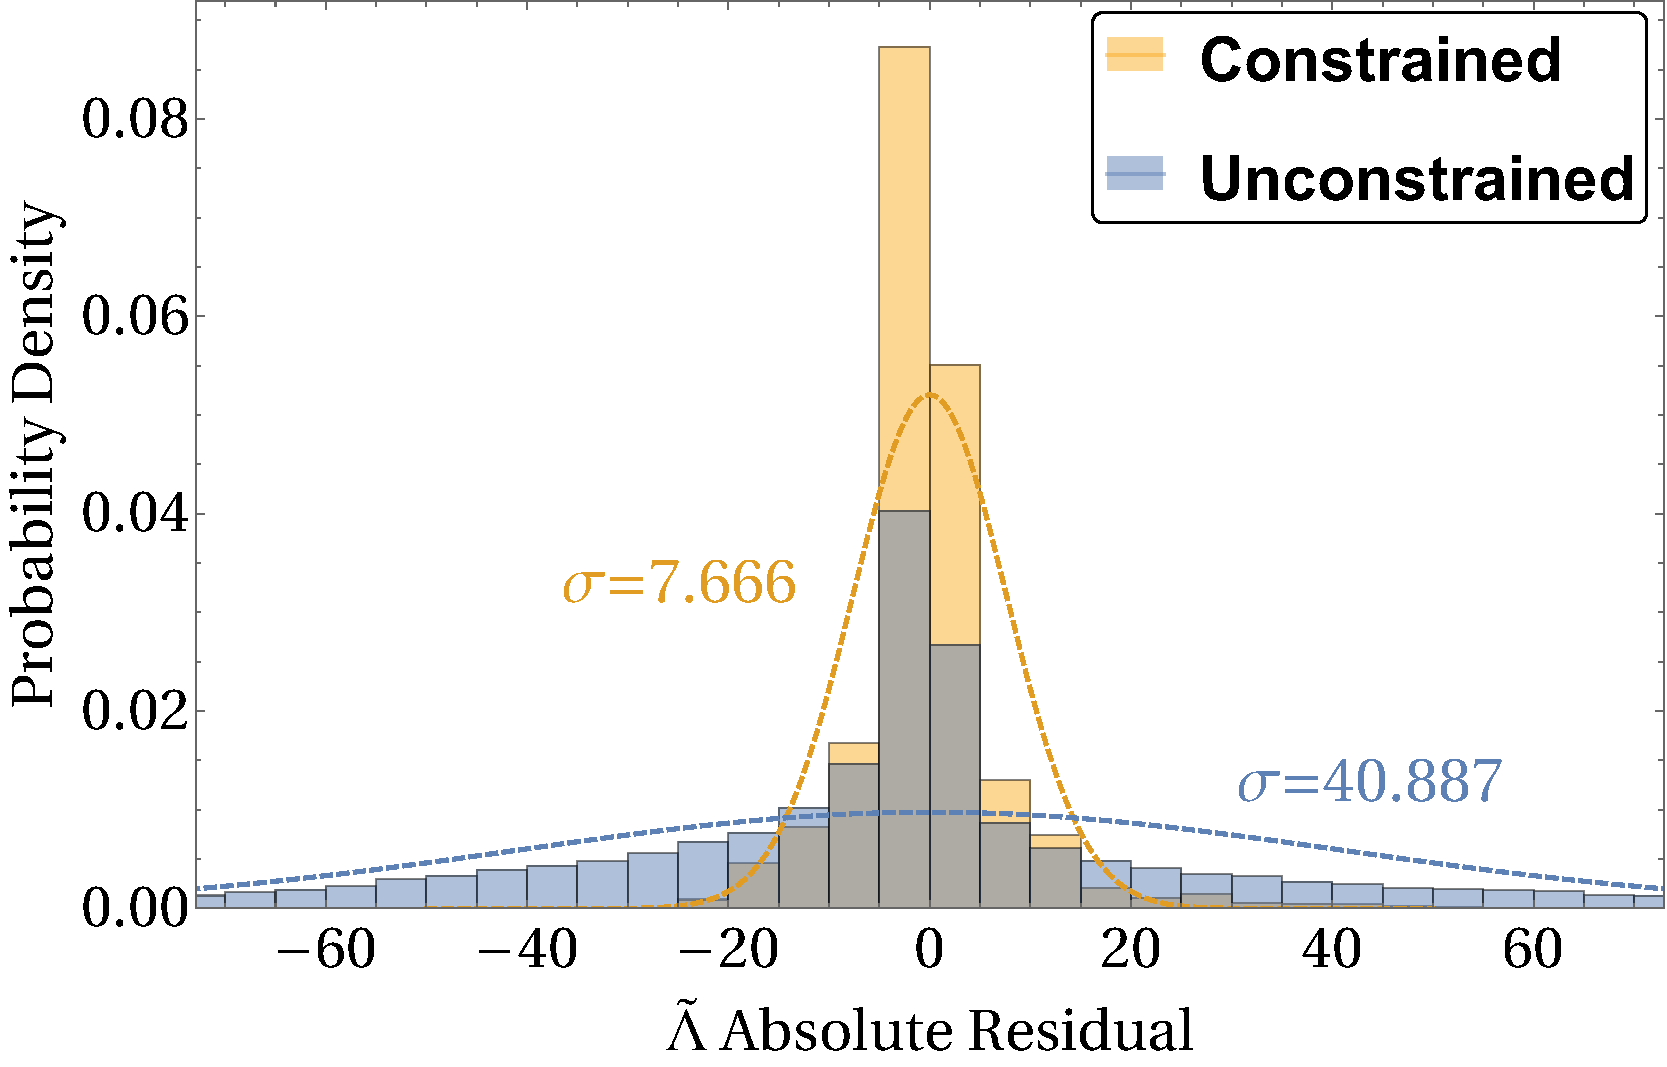
\includegraphics[width=\columnwidth]{residuals.pdf}
\end{center}
\caption{
Residuals on $\tilde\Lambda$ computed as $\tilde{\Lambda}^{\text{fit}}-\tilde{\Lambda}^{\text{true}}$ for the binary Love relations modeled in Sec.~\ref{sec:binLove-nuclear} for both constrained and unconstrained sets of EoSs.
These residuals obey Gaussian distributions centered at $\mu=-1.8133 \times 10^{-4}$ and $\mu=4.2258 \times 10^{-3}$ with standard deviations of $\sigma=7.6664$ and $\sigma=40.8866$ for the constrained and unconstrained sets of EoSs, respectively.
These uncertainties correspond roughly to the systematic errors introduced on the parameter extraction of $\tilde{\Lambda}$ upon the use of binary Love universal relations.
However, to take into account the systematic errors found in high-error regions of the parameter space, we instead set the systematic error to be the 90th percentile, $P_{90}=12.014$.
Observe that the systematic errors from using the improved (constrained) binary Love universal relations are negligible compared to the statistical errors accrued on parameter extraction from GW170817, found to be $\sigma_{\tilde{\Lambda}}=198$.
}
\label{fig:residuals}
\end{figure}

%%%%%%%%%%%%%%%%%%%%%%%%% Begin Future Observations %%%%%%%%%%%%%%%%%%%%%%%%%%%%%%%%%%%%%%%%%%%%%%%%%%%%%%%%%%%%%%%%%%%%%%%%%%%%%%%%%%%%%%%%%%%%%%%%%%%%%%%%%%%%%%%%%%%%%%%%%%%%%%%%%%%%%%%%%%%%%%%%%%%%%
\section{Impact on future observations}\label{sec:observations}
In this section, we estimate the feasibility of utilizing improved universal relations in future binary NS merger events.
This estimate is acquired through a simple Fisher analysis~\cite{Finn:Fisher,Cutler:Fisher} which approximates the accuracy with which one can extract best-fit parameters $\theta^a$, given a prior template waveform.
For the remainder of the paper, we consider a template parameter vector consisting of:
\begin{equation}\label{eq:template}
\theta^a=(\ln{A},\phi_c,t_c,\ln{\mathcal{M}},\ln{\mathcal{\eta}},\chi_s,\chi_a,\tilde{\Lambda},\delta \tilde{\Lambda}),
\end{equation}
where $A \equiv \sqrt{\frac{2 \eta}{3 \pi^{1/3}}}$ is a normalized amplitude factor, $\eta \equiv m_1 m_2/M^2$ is the symmetric mass ratio with $m_{1,2}$ and $M$ being the individual and total masses, $\mathcal{M}=M \eta^{3/5}$ is the chirp mass, and $\chi_{s,a}=\frac{1}{2}(\chi_1\pm\chi_2)$ are the symmetric and antisymmetric total spins, where $\chi_{1,2}$ are the NSs individual spins. 
Following Refs.~\cite{Cutler:Fisher,Berti:Fisher,Poisson:Fisher}, this method relies on the crude assumption of Gaussian prior distributions\footnote{Typically, the more valid assumption is a uniform prior distribution; an improvement made in a more detailed Bayesian analysis.}.
The resulting posterior distribution is Gaussian with root-mean-square given by:
\begin{equation}
\Delta \theta^a=\sqrt{\Big( \tilde{\Gamma}^{-1}\Big)^{aa}}.
\end{equation}
Here, the Fisher matrix $\tilde{\Gamma}$ is defined by:
\begin{equation}
\tilde{\Gamma}_{ab} \equiv \Big( \frac{\partial h}{\partial \theta^a} \Big| \frac{\partial h}{\partial \theta^a}\Big) + \frac{1}{\sigma_{\theta^a}^2} \delta_{ab}
\end{equation}
where $h$ is the waveform template, $\sigma_{\theta^a}$ is the parameters' prior root-mean-square estimate, and the inner product is defined by:
\begin{equation}
(a|b) \equiv 2 \int^{\infty}_0\frac{\tilde{a}^*\tilde{b}+\tilde{b}^*\tilde{a}}{S_n(f)}df.
\end{equation}
In this analysis, we consider the ``PhenomD" waveform template~\cite{PhenomDI,PhenomDII} modified by tidal corrections shown in Ref.~\cite{Wade:tidalCorrections}.
Lastly, $S_n(f)$ is the spectral noise density for the given interferometer.

We begin by authenticating this approach by applying a Fisher analysis to GW170817, as observed by LIGO with O2 detector sensitivity\zc{cite}.
Further, we scale the luminosity distance such that the signal-to-noise-ratio ($SNR \equiv \rho$) is fixed to be $\rho=32.4$, as was found in GW170817.
We also assume low spin priors $|\chi| \leq 0.05$, as well as $\tilde{\Lambda} \leq 3000$ and $|\delta \tilde{\Lambda}| \leq 500$~\cite{Wade:LambdaPriors}.
The resulting posterior distribution on $\tilde{\Lambda}$ has a range of $\pm 276.99$ encompassing the $90\%$ credible levels.
We compare these results with the Bayesian analysis performed in Ref.~\cite{TheLIGOScientific:2017qsa,Abbott2018}, finding close agreement with the resulting $90\%$ credible region of $70 \leq \tilde{\Lambda} \leq 720$.
This confirms the approximate validity of this method, allowing a continuation of this analysis for future detectors.
\begin{figure}
\begin{center} 
\includegraphics[width=\columnwidth]{sensitivities.eps}
\end{center}
\caption{
Square root of of the spectral noise densities $\sqrt{S_n^A(f)}$ plotted for detectors ($A$): LIGO O2 (orange), aLIGO (green), a\texttt{++} (purple), Voyager (magenta), CE (red), and ET-D (blue) as interpolated from publicly available data\zc{cite}.
Spectral noise densities are plotted from $f_{\text{min}}=(23,10,10,7,1,1) \text{ Hz}$, respectively, to $f_{\text{max}}=1649 \text{ Hz}$.
Also shown is $2 \sqrt{f}$ multiplied by the amplitude of the PhenomD~\cite{PhenomDI,PhenomDII} waveform template, modified by tidal corrections from Ref.~\cite{Wade:tidalCorrections} used in our Fisher Analysis.
}
\label{fig:sensitivities}
\end{figure}

Next, we consider events identical to GW170817 detected on future design sensitivity upgrades and detectors $A \equiv ($O2, aLIGO, a\texttt{++}, Voyager, CE, ET-D$)$\zc{cite}, shown in Fig.~\ref{fig:sensitivities}, to determine if and when the statistical errors associated with parameter extraction of $\tilde{\Lambda}$ drop below the systematic EoS variation errors from using binary Love universal relations.
The process we use for each detector sensitivity $S_n^A(f)$ is as follows:
\begin{itemize}
\item Perform a Fisher analysis as outlined above using $S_n^A(f)$, while restricting the luminosity distance $D_L$ such that $\rho^{\text{O2}}_{\text{GW170817}}=32.4$ would be achieved on O2 sensitivity $S_n^{\text{O2}}(f)$.
This results in SNR $\rho^A_{\text{GW170817}}$ and statistical error $\sigma_\text{GW170817}^A$ accrued in the extraction of $\tilde{\Lambda}$ on detector $A$.
\item Generate a population of $N_A$ events corresponding to the expected binary NS merger detection rate for detector $A$, following the distribution $f=3 \rho_{\text{th}}^3/\rho^4$~\cite{Shutz:SNR,Chen:SNR} with a network SNR threshold of $\rho_{\text{th}}=8$.
This is calculated for the upper, central, and lower limits of the local binary NS coalescence rate density $R=1540^{+3200}_{-1220} \text{ Gpc}^{-3}\text{yr}^{-1}$~\cite{Abbott2017}, giving the rates shown in the second column of Table~\ref{tab:variances}.
\item Compute the population standard deviation given by:
\begin{equation}
\frac{1}{(\sigma_N^A)^2}=\sum_i^{N_A}\frac{1}{(\sigma_i^A)^2},
\end{equation}
where $\sigma_i^A$ is computed by the relations $\sigma_i^A \times \rho_i^A = \sigma_{\text{GW170817}}^A \times \rho_{\text{GW170817}}^A$.
\end{itemize}
The results are compiled in Table~\ref{tab:variances}, and shown graphically in Fig.~\ref{fig:stackedFisher} where $\sigma^A_{\text{GW170817}}$ and $\sigma^A_N$ are plotted as a function of $\rho^A_{\text{GW170817}}$ (the SNR as if GW170817 were detected on future detector $A$) for 5 future detector sensitivities.

\begin{table*}
\centering
\caption{
Tabulated results for the estimated statistical errors on $\tilde{\Lambda}$ for the combined results of $N_A$ detections corresponding to the estimated upper, central, and lower limits of the binary NS merger detection rate $R$.
This is repeated for 5 future detector sensitivities: aLIGO, a\texttt{++}, Voyager, CE, and ET.
Below, $\rho^A_{\text{GW170817}}$ and $\sigma^A_{\text{GW170817}}$ correspond to the approximate SNR and $\sigma_{\tilde{\Lambda}}$ of GW170817 had it been observed by the future interferometer, and $\sigma^A_N$ corresponds to the final uncertainty on $\tilde{\Lambda}$ after $N_A$ detections on interferometer $A$.
It can be seen here that the statistical errors on $\tilde{\Lambda}$ become comparable with the systematics (set to be $P_{90}=12.014$) from using improved binary Love relations from Voyager and on, indicating when it may be safe to utilize new universal relations.
Note the approximation for $\sigma^A_N$ under the O2 detector sensitivity is left blank due to the singularity of the detected event.
These results are shown graphically in Fig.~\ref{fig:stackedFisher}.
}\label{tab:variances}
%\begin{tabular}{ c || c c c c c c c c} 
%\hline
%Detector ($A$) & $N_A (\text{Lower})$ & $N_A (\text{Central})$ & $N_A (\text{Upper})$ & $\rho^A_{\text{GW170817}}$ & $\sigma^A_{\text{GW170817}}$ & $\sigma^A_N (\text{Lower})$ & $\sigma^A_N (\text{Central})$ & $\sigma^A_N (\text{Upper})$\\
%\hline
%\hline
%O2 & $1$ & $1$ & $1$ & $32.40$ & $168.40$ & $558.18$ & $393.24$ & $279.44$\\
%aLIGO & $23$ & $112$ & $344$ & $90.74$ & $75.44$ & $117.022$ & $42.89$ & $24.27$\\
%a\texttt{++} & $208$ & $1004$ & $3091$              & $180.95$ & $31.55$ &               $27.62$ & $13.36$ & $7.36$\\
%Voyager & $3854$ & $1.85 \times 10^4$ & $5.71 \times 10^4$ &              $428.89$ & $16.69$              & $8.57$ & $3.78$ & $2.16$\\
%ET-D & $3.98\times 10^5$ & $1.91\times 10^6$ & $5.89\times 10^6$ &                  $2807.45$ & $6.26$ &               $0.78$ & $0.35$ & $0.20$\\
%CE & $1.35\times 10^7$ & $6.50\times 10^7$ & $2.00\times 10^8$ &                 $1398.03$ & $4.85$ &                 $0.34$ & $0.16$ & $0.10$\\
%\hline
%\end{tabular}
\begin{tabular}{|c|@{\extracolsep{4pt}}c@{\extracolsep{0pt}}|c|@{\extracolsep{4pt}}C{1.7cm}@{\extracolsep{-2pt}}|C{1.7cm}|@{\extracolsep{-2pt}}C{1.7cm}@{\extracolsep{2pt}}|c|@{\extracolsep{0pt}}c@{\extracolsep{0pt}}|c|}
\cline{1-1}\cline{2-3}\cline{4-9}
    \multicolumn{1}{|c|}{\bfseries Detectors (A)} & \multicolumn{2}{|c|}{\bfseries GW170817} & \multicolumn{6}{|c|}{\bfseries Multiple events} \\
\cline{1-1}\cline{2-3}\cline{4-9}
\noalign{\smallskip}
\cline{2-3}\cline{4-6}\cline{7-9}
\multicolumn{1}{c}{} & \multicolumn{1}{|c|}{} & \multicolumn{1}{c|}{} & \multicolumn{3}{|c|}{} & \multicolumn{3}{|c|}{}
\\[-1em]
\multicolumn{1}{c}{}  &  \multicolumn{1}{|c|}{\multirow{2}{*}{$\rho^A_{\text{GW170817}}$}}  &  \multirow{ 2}{*}{$\sigma^A_{\text{GW170817}}$}  &  \multicolumn{3}{|c|}{$N_A$}  &  \multicolumn{3}{|c|}{$\sigma^A_N$}  \\
\cline{4-6}\cline{7-9}
\multicolumn{1}{c}{}  &  \multicolumn{1}{|c|}{}  &  \multicolumn{1}{c|}{}  &  \multicolumn{1}{|c|}{Low}  &  \multicolumn{1}{c|}{Central} &  \multicolumn{1}{c|}{High}  & \multicolumn{1}{|c|}{Low}  &  \multicolumn{1}{c|}{Central} &  \multicolumn{1}{c|}{High}\\
\cline{2-3}\cline{4-6}\cline{7-9}
\noalign{\smallskip}
\noalign{\smallskip}
\cline{1-1}\cline{2-3}\cline{4-6}\cline{7-9}
 O2  & \multicolumn{1}{|c|}{$32.40$}  & $168.40$ &  \multicolumn{1}{|c|}{--} & -- & -- & \multicolumn{1}{|c|}{--} & -- & --\\
\cline{1-1}\cline{2-3}\cline{4-6}\cline{7-9}
 aLIGO  & \multicolumn{1}{|c|}{$90.74$}  & $75.44$ &  \multicolumn{1}{|c|}{$23$} & $112$ & $344$ & \multicolumn{1}{|c|}{$117.022$} & $42.89$ & $24.27$\\
\cline{1-1}\cline{2-3}\cline{4-6}\cline{7-9}
 a\texttt{++}  & \multicolumn{1}{|c|}{$180.95$}  & $31.55$ &  \multicolumn{1}{|c|}{$208$} & $1004$ & $3091$ & \multicolumn{1}{|c|}{$27.62$} & $13.36$ & $7.36$\\
\cline{1-1}\cline{2-3}\cline{4-6}\cline{7-9}

\multicolumn{1}{|c|}{} & \multicolumn{1}{|c|}{} & \multicolumn{1}{c|}{} & \multicolumn{1}{|c|}{} & \multicolumn{1}{c|}{} & \multicolumn{1}{c|}{} & \multicolumn{1}{|c|}{} & \multicolumn{1}{c|}{} & \multicolumn{1}{c|}{}
\\[-1em]

 Voyager  & \multicolumn{1}{|c|}{$428.89$}  & $16.69$ &  \multicolumn{1}{|c|}{$3854$} & $1.85 \times 10^4$ & $5.71 \times 10^4$ & \multicolumn{1}{|c|}{$8.57$} & $3.78$ & $2.16$\\
\cline{1-1}\cline{2-3}\cline{4-6}\cline{7-9}

\multicolumn{1}{|c|}{} & \multicolumn{1}{|c|}{} & \multicolumn{1}{c|}{} & \multicolumn{1}{|c|}{} & \multicolumn{1}{c|}{} & \multicolumn{1}{c|}{} & \multicolumn{1}{|c|}{} & \multicolumn{1}{c|}{} & \multicolumn{1}{c|}{}
\\[-1em]

 ET-D  & \multicolumn{1}{|c|}{$2807.45$}  & $6.26$ &  \multicolumn{1}{|c|}{$3.98 \times 10^5$} & $1.91 \times 10^6$ & $5.89 \times 10^6$ & \multicolumn{1}{|c|}{$0.78$} & $0.35$ & $0.20$\\
\cline{1-1}\cline{2-3}\cline{4-6}\cline{7-9}

\multicolumn{1}{|c|}{} & \multicolumn{1}{|c|}{} & \multicolumn{1}{c|}{} & \multicolumn{1}{|c|}{} & \multicolumn{1}{c|}{} & \multicolumn{1}{c|}{} & \multicolumn{1}{|c|}{} & \multicolumn{1}{c|}{} & \multicolumn{1}{c|}{}
\\[-1em]

 CE  & \multicolumn{1}{|c|}{$1398.03$}  & $4.85$ &  \multicolumn{1}{|c|}{$1.35 \times 10^7$} & $6.50 \times 10^7$ & $2.00 \times 10^8$ & \multicolumn{1}{|c|}{$0.34$} & $0.16$ & $0.10$\\
\cline{1-1}\cline{2-3}\cline{4-6}\cline{7-9}
\end{tabular}
\end{table*}

Concluding, we find that the Voyager, ET, and CE detectors all exhibit enough uncertainty reduction that the systematics on $\tilde\Lambda$ introduced from using improved universal relations (found to be $12.014$) no longer become negligible in the error budget.
This implies that the use and further improvement of universal relations is justified for future binary NS merger detections.
Further, we investigate the dependence of the measurement accuracy of $\tilde\Lambda$ on the binary NS mass ratio $q$ for fixed chirp mass $\mathcal{M}=1.88\text{ M}_{\odot}$ in Appendix~\ref{app:measurement}.

%%%%%%%%%%%%%%%%%%%%%%%%% Begin Discussion %%%%%%%%%%%%%%%%%%%%%%%%%%%%%%%%%%%%%%%%%%%%%%%%%%%%%%%%%%%%%%%%%%%%%%%%%%%%%%%%%%%%%%%%%%%%%%%%%%%%%%%%%%%%%%%%%%%%%%%%%%%%%%%%%%%%%%%%%%%%%%%%%%%%%
\section{Conclusion and Discussion}\label{sec:conclusion}
The recent GW observation of binary NS merger GW170817 placed constraints on the supranuclear matter EoS for NSs.
We take advantage of this by generating a restricted set of spectral EoSs which agree with this observation to reduce uncertainties upon the extraction of tidal parameters from future GW events.
Important previous work by Yagi and Yunes~\cite{Yagi:ILQ,Yagi:binLove} found EoS-insensitive universal relations between symmetric and antisymmetric combinations of NS tidal deformabilities, which aid in the extraction of said tidal parameters.
We find an improvement upon these universal relations by a factor of $\sim 59$\% for stars with mass ratios of $0.75$ by restricting to the EoS posterior samples from GW170817s 90\% credible region on pressure as a function of density.
Similarly, we find an increase in I-Love-Q universality by a factors of $\sim 50$\%.
In addition, we find that binaries consisting of one massive hybrid quark-hadron star, and one small-mass hadron star do not obey these universal relations -- explained by the large difference in $\tilde{\Lambda}$ displayed between the constituent stars.
To improve on this, we construct new ``hybrid matter binary Love relations", applied to only the hybrid branches of the transitional EoSs.
This results in EoS variability similar to that found for the nuclear matter fits.
Further, we analyze the impact of this improvement for future binary NS merger detections, as the current detector sensitivity is not yet small enough to accurately constrain $\tilde{\Lambda}$ enough for universal relations to make a difference.
We find that future interferometers Voyager, CE, and ET-D all experience statistical uncertainties upon the extraction of $\tilde{\Lambda}$ small enough to become comparable to the systematic errors injected through the use of improved universal relations (found to be $12.014$), as depicted in Fig.~\ref{fig:stackedFisher} and Table~\ref{tab:variances}.
Finally, in Appendix~\ref{app:measurement} we investigate the effect of NS binary mass ratio q on the measurement accuracy of $\tilde\Lambda$.
We find that second generation interferometers lose accuracy as one increases the mass ratio, while third generation detectors observe a large increase of accuracy due to the correlations between $\tilde\Lambda$ and $\delta\tilde\Lambda$.
This indicates that the use and further improvement of universal relations is justified for future GW observations of binary NS merger events.

\zc{Discuss with group on possible avenues of future work.}

%%%%%%%%%%%%%%%%%%%%%%%%% Begin Acknowledgements %%%%%%%%%%%%%%%%%%%%%%%%%%%%%%%%%%%%%%%%%%%%%%%%%%%%%%%%%%%%%%%%%%%%%%%%%%%%%%%%%%%%%%%%%%%%%%%%%%%%%%%%%%%%%%%%%%%%%%%%%%%%%%%%%%%%%%%%%%%%%%%%%%%%%
\section*{Acknowledgments}\label{acknowledgments}
K.Y. would like to acknowledge networking support by the COST Action GWverse CA16104.


%%%%%%%%%%%%%%%%%%%%%%%%% Begin Appendix A: measurement accuracy as a functino of q %%%%%%%%%%%%%%%%%%%%%%%%%%%%%%%%%%%%%%%%%%%%%%%%%%%%%%%%%%%%%%%%%%%%%%%%%%%%%%%%%%%%%%%%%%%%%%%%%%%%%%%%%%%%%%%%%%%%%%%%%%%%%%%%%%%%%%%%%%%%%%%%%%%%%
\appendix
\section{Measurement accuracy as a function of binary mass ratio}\label{app:measurement}
In this appendix, we discuss the effects of the binary NS mass ratio on the measurement accuracy of $\tilde\Lambda$ for various interferometers. 
The left panel of Fig.~\ref{fig:massVariation} displays an approximation of the $\tilde\Lambda$ measurement accuracy as a function of increasing mass ratio $q$ (for a fixed chirp mass of $\mathcal{M}=1.188 \text{ M}_{\odot}$ corresponding to GW170817), using the Fisher analysis techniques described in Sec.~\ref{sec:observations}.
We observe two points of interest about these trends: (i) the second generation detectors (O2, aLIGO, a\texttt{++}, and Voyager) typically become less accurate as the mass ratio approaches unity, (ii) the third generation detectors (CE and ET) observe the opposite behavior-- a fast growth in accuracy as the mass ratio increases.
For the remainder of this appendix, we attempt to explain the opposing behaviors of the second and third generation interferometers on the extraction of $\tilde\Lambda$.

\begin{figure*}
\begin{center} 
\includegraphics[width=.3\textwidth]{massVariation1.eps}
\includegraphics[width=.3\textwidth]{massVariation2.eps}
\includegraphics[width=.3\textwidth]{massVariation3.eps}
\end{center}
\caption{
Measurement accuracy of $\tilde\Lambda$ as a function of increasing mass ratio $q$ for interferometer sensitivities O2, aLIGO, a\texttt{++}, Voyager, CE, and ET.
Evaluated at a fixed chirp mass of $\mathcal{M}=1.188\text{ M}_{\odot}$ corresponding to GW170817, this is repeated for three cases: (i) (left) with correlations between all template waveform parameters $\theta^a$ intact; (ii) (center) with the correlations between $\tilde\Lambda$ and $\delta\tilde\Lambda$ removed; and (iii) (right) with correlations between all parameters removed.
The removal of parameter correlations is approximated by setting certain Fisher matrix elements to 0, as described in Appendix.~\ref{app:measurement}.
Observe how the left panel shows strong disagreement between second and third generation detectors, while the right panel shows identical behavior.
This indicates that parameter correlations between $\tilde\Lambda$ and higher PN order parameter $\delta\tilde\Lambda$ to be the culprit in such a disagreement.
}
\label{fig:massVariation}
\end{figure*} 

We begin by considering the correlations between individual template parameters and $\tilde\Lambda$, given in Eq.~\ref{eq:template}.
A simple approximation on the amplitude of these correlations can be performed by assuming all other correlations are non-existing.
Correlations between parameters $\tilde\Lambda$ and $\theta^a$ alone is achieved by setting all off-diagonal Fisher matrix elements to $0$, except for the $(i,j)$ components such that both $i$ and $j$ correspond to the $\tilde\Lambda$ and $\theta^a$ parameters.
We follow this process for each parameter in turn, and display the results in Fig.~\ref{fig:correlations} for each interferometer.
This figure, showing only the relative differences between correlations of different parameters $\theta^a$ and $\tilde\Lambda$, reveals a few things.
First, the coalescence time $t_c$ is highly correlated with $\tilde\Lambda$ equally for each interferometer, an unsurprising fact due to the high 4PN order at which the parameter enters the waveform.
Secondly, correlations with 6PN tidal parameter $\delta\tilde\Lambda$ shows high correlations with $\tilde\Lambda$ for only the third generation detectors.
This can be explained by the high PN order at which $\delta\tilde\Lambda$ enters the waveform, an effect that only the most sensitive of detectors can probe. 

\begin{figure}
\begin{center} 
\begin{overpic}[width=\columnwidth]{correlations.eps}
\put(121,13){\fontsize{7pt}{7pt}\selectfont $\mathcal{M}$}
\end{overpic}
\end{center}
\caption{
Measurement accuracy of $\tilde\Lambda$ upon the consideration of correlations between \emph{only} $\tilde\Lambda$ and other individual template parameters $\theta^a$ shown in Eq.~\ref{eq:template}.
This process, repeated for 6 interferometer design sensitivities O2, aLIGO, a\texttt{++}, Voyager, CE, and ET, is approximated by setting all off-diagonal Fisher matrix elements to 0 except for the $(i,j)$ components such that both $i$ and $j$ correspond to the $\tilde\Lambda$ and $\theta^a$ parameters.
Observe how correlations with 4PN parameter $t_c$ (coalescence time) remain to be highly correlated with $\tilde\Lambda$ among all 6 interferometers.
However, correlations between 6PN tidal parameter $\delta\tilde\Lambda$ and $\tilde\Lambda$ only begin to make a strong impact for third generation detectors.
This is due to the small effect that $\delta\tilde\Lambda$ has on the waveform, only to be distinguished by the most sensitive detectors.
}
\label{fig:correlations}
\end{figure} 

Following this conclusion on the difference of correlations between tidal parameters $\tilde\Lambda$ and $\delta\tilde\Lambda$ for second and third generation detectors, we attempt to describe the opposing behaviors of measurement accuracy between the two.
Shown in the center panel of Fig.~\ref{fig:massVariation}, we approximate the measurement accuracy of $\tilde\Lambda$ with the correlations between $\delta\tilde\Lambda$ and $\tilde\Lambda$ removed, through a process similar to that described above. 
Notice how the trends between detector generations become more similar -- implying that the correlations between tidal parameters may be the cause.
This is confirmed by the right panel of Fig.~\ref{fig:massVariation} where all parameter correlations have been removed from the Fisher matrix.
We see that this results in identical behaviors between all 6 representative interferometers, leading us to conclude that the discrepancy between interferometers comes from the degeneracies between different parameters in the gravitational waveform, namely the 6PN tidal parameter $\delta\tilde\Lambda$ which is only detectable by the highly sensitive third generation detectors CE and ET.

%%%%%%%%%%%%%%%%%%%%%%%%% Begin Bibliography  %%%%%%%%%%%%%%%%%%%%%%%%%%%%%%%%%%%%%%%%%%%%%%%%%%%%%%%%%%%%%%%%%%%%%%%%%%%%%%%%%%%%%%%%%%%%%%%%%%%%%%%%%%%%%%%%%%%%%%%%%%%%%%%%%%%%%%%%%%%%%%%%%%%%%
\clearpage
\bibliography{Zack}
\end{document}

